\documentclass{article}

\usepackage[utf8x]{inputenc}
\usepackage[T1]{fontenc}
\usepackage[latin1]{inputenc}
\usepackage{eurosym}
\usepackage[version=3]{mhchem} 
\usepackage{siunitx}
\usepackage{graphicx}
\usepackage{natbib} 
\usepackage{amsmath} 

\setlength\parindent{0pt} 
\renewcommand{\labelenumi}{\alph{enumi}.} 

\title{Vision stéréoscopique \\ POO 2} 
\date{10 décembre 2014}
\author{Benjamin Chetioui   Clément Schreiner   Loic Laisne}

\begin{document}

\maketitle

\begin{center}
\begin{tabular}{l r}
Date de la présentation: & 10 Décembre 2014 \\ 
Correcteur: & Benoît Sonntag 
\end{tabular}
\end{center}

\section{Présentation}

L’objectif de ce projet est de construire une representation en 3D d’un objet réél à partir d'images en deux dimensions d’un même objet.\\
Le programme comportera une interface graphique.


\subsection{Choix du langage, choix de librairies}
Pour réaliser ce projet, nous avons choisi d'utiliser les langages C++ et Lisaac.\\
Pour l'interface, nous utilisons la librairie QT.
 
\subsection{Choix et simplifications personnelles du sujet}

 Nous avons décidé de séparer le projet en deux programmes : \\
 \begin{tabular} - - Un qui gére l'interface utilisateur pour indiquer les points de correspondance à la souris (C++) \end{tabular}\\
 \begin{tabular} - - Un qui gére l'affichage 3D et la stéréovision (Lisaac) \end{tabular}
 
\subsection{Répartition des tâches}
Nous nous sommes réparti les tâches comme suit : \\
\begin{tabular} - CHETIOUI Benjamin : les prototypes Modes, Translate, Triangulate (Lisaac)\end{tabular}\\
\begin{tabular} - LAISNE Loïc : les Prototypes Point, Lines et Depth (Lisaac)\end{tabular}\\
\begin{tabular} - SCHREINER Clément : Interface (C++)\end{tabular}\\
La répartition ci-dessus n'est pas représentative : chacun a participé à toutes les parties du code.\\

\newpage

\section{Diagrammes de classes}
Veuillez trouver ci-dessous les deux diagrammes de classes du projet
\\ \\
\begin{figure}[h]
\begin{center}
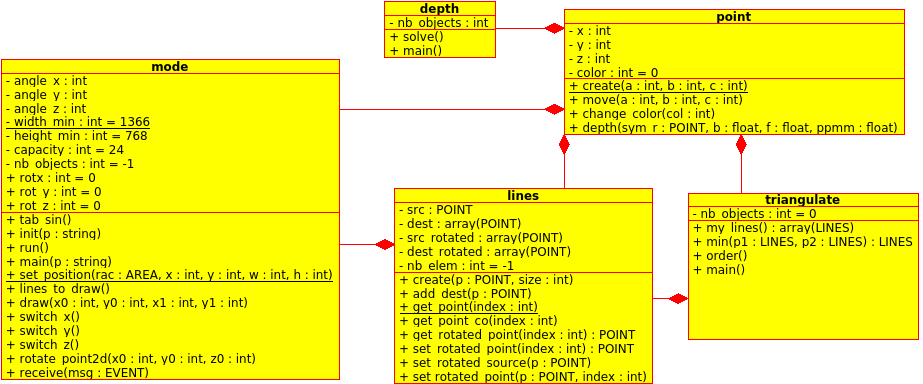
\includegraphics[width=0.65\textwidth]{diag_classes.png}
\caption{Diagramme de classe - interface}
\end{center}
\end{figure}
\\ \\
\begin{figure}[h]
\begin{center}
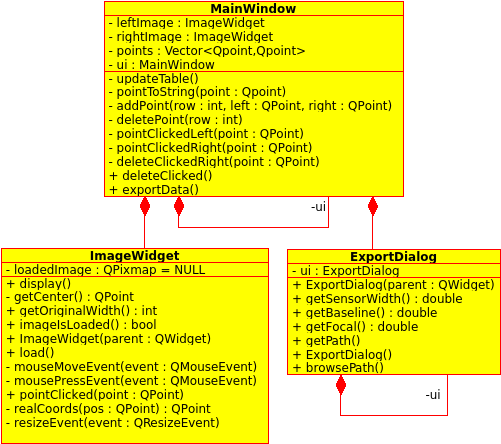
\includegraphics[width=0.65\textwidth]{diag_classes_gui}
\caption{Diagramme de classe - Stéréovision}
\end{center}
\end{figure}

\newpage

\section{Algorithmes}
  
\subsection{Calcul profondeur - Point}

\subsection{Algorithme de triangulation (SOON !!!)} 

\end{document}
